El diagrama de la Figura~\ref{fig:vista-general}, Vista General en Capas, constituye una representación arquitectónica en ArchiMate que organiza y jerarquiza la interacción entre los distintos niveles de abstracción que sostienen la provisión de servicios de ejecución de contenedores. En la capa de actores externos se identifican los roles de investigador y estudiante, los cuales, a través de proyectos institucionales, demandan servicios de negocio tales como autenticación, autorización y acceso a recursos, configurando así la relación entre los objetivos académicos y los mecanismos tecnológicos de soporte. Estos servicios habilitan el proceso de negocio de “Ejecución de contenedores”, que se desglosa en las fases —registro, validación, asignación de recursos y despliegue—, evidenciando una lógica de orquestación que articula tanto el flujo de requerimientos como la satisfacción de las necesidades de los usuarios. Dicha capa de negocio se conecta con servicios de aplicación externos como firewalls, internet e IPs públicas, lo que refleja la dependencia del ecosistema en infraestructuras de conectividad seguras y abiertas. A nivel de componentes de aplicación, el diagrama detalla la función de K3S, Kubelet, Containerd y archivos de configuración YML, los cuales actúan como mediadores técnicos entre las solicitudes de alto nivel y la ejecución efectiva en los entornos virtualizados, integrando estándares de orquestación de contenedores propios de Kubernetes. Esta lógica se apoya en servicios de infraestructura externos —Docker Hub y repositorios APT— que proveen tanto imágenes de contenedores como dependencias necesarias para la reproducibilidad y consistencia de los entornos desplegados. Finalmente, en la capa de infraestructura física se sitúan los elementos tangibles que fundamentan el ecosistema: racks con hipervisores XCP-NG que ejecutan máquinas virtuales y sistemas de almacenamiento \NAS, configurando una plataforma híbrida que combina virtualización, contenedorización y aprovisionamiento dinámico de recursos. En conjunto, el diagrama no solo presenta una visión técnica integral, sino que también establece una correspondencia clara entre los objetivos estratégicos de investigación académica y la materialización tecnológica de un entorno flexible, escalable y seguro.
\begin{figure}[H]
    \centering
    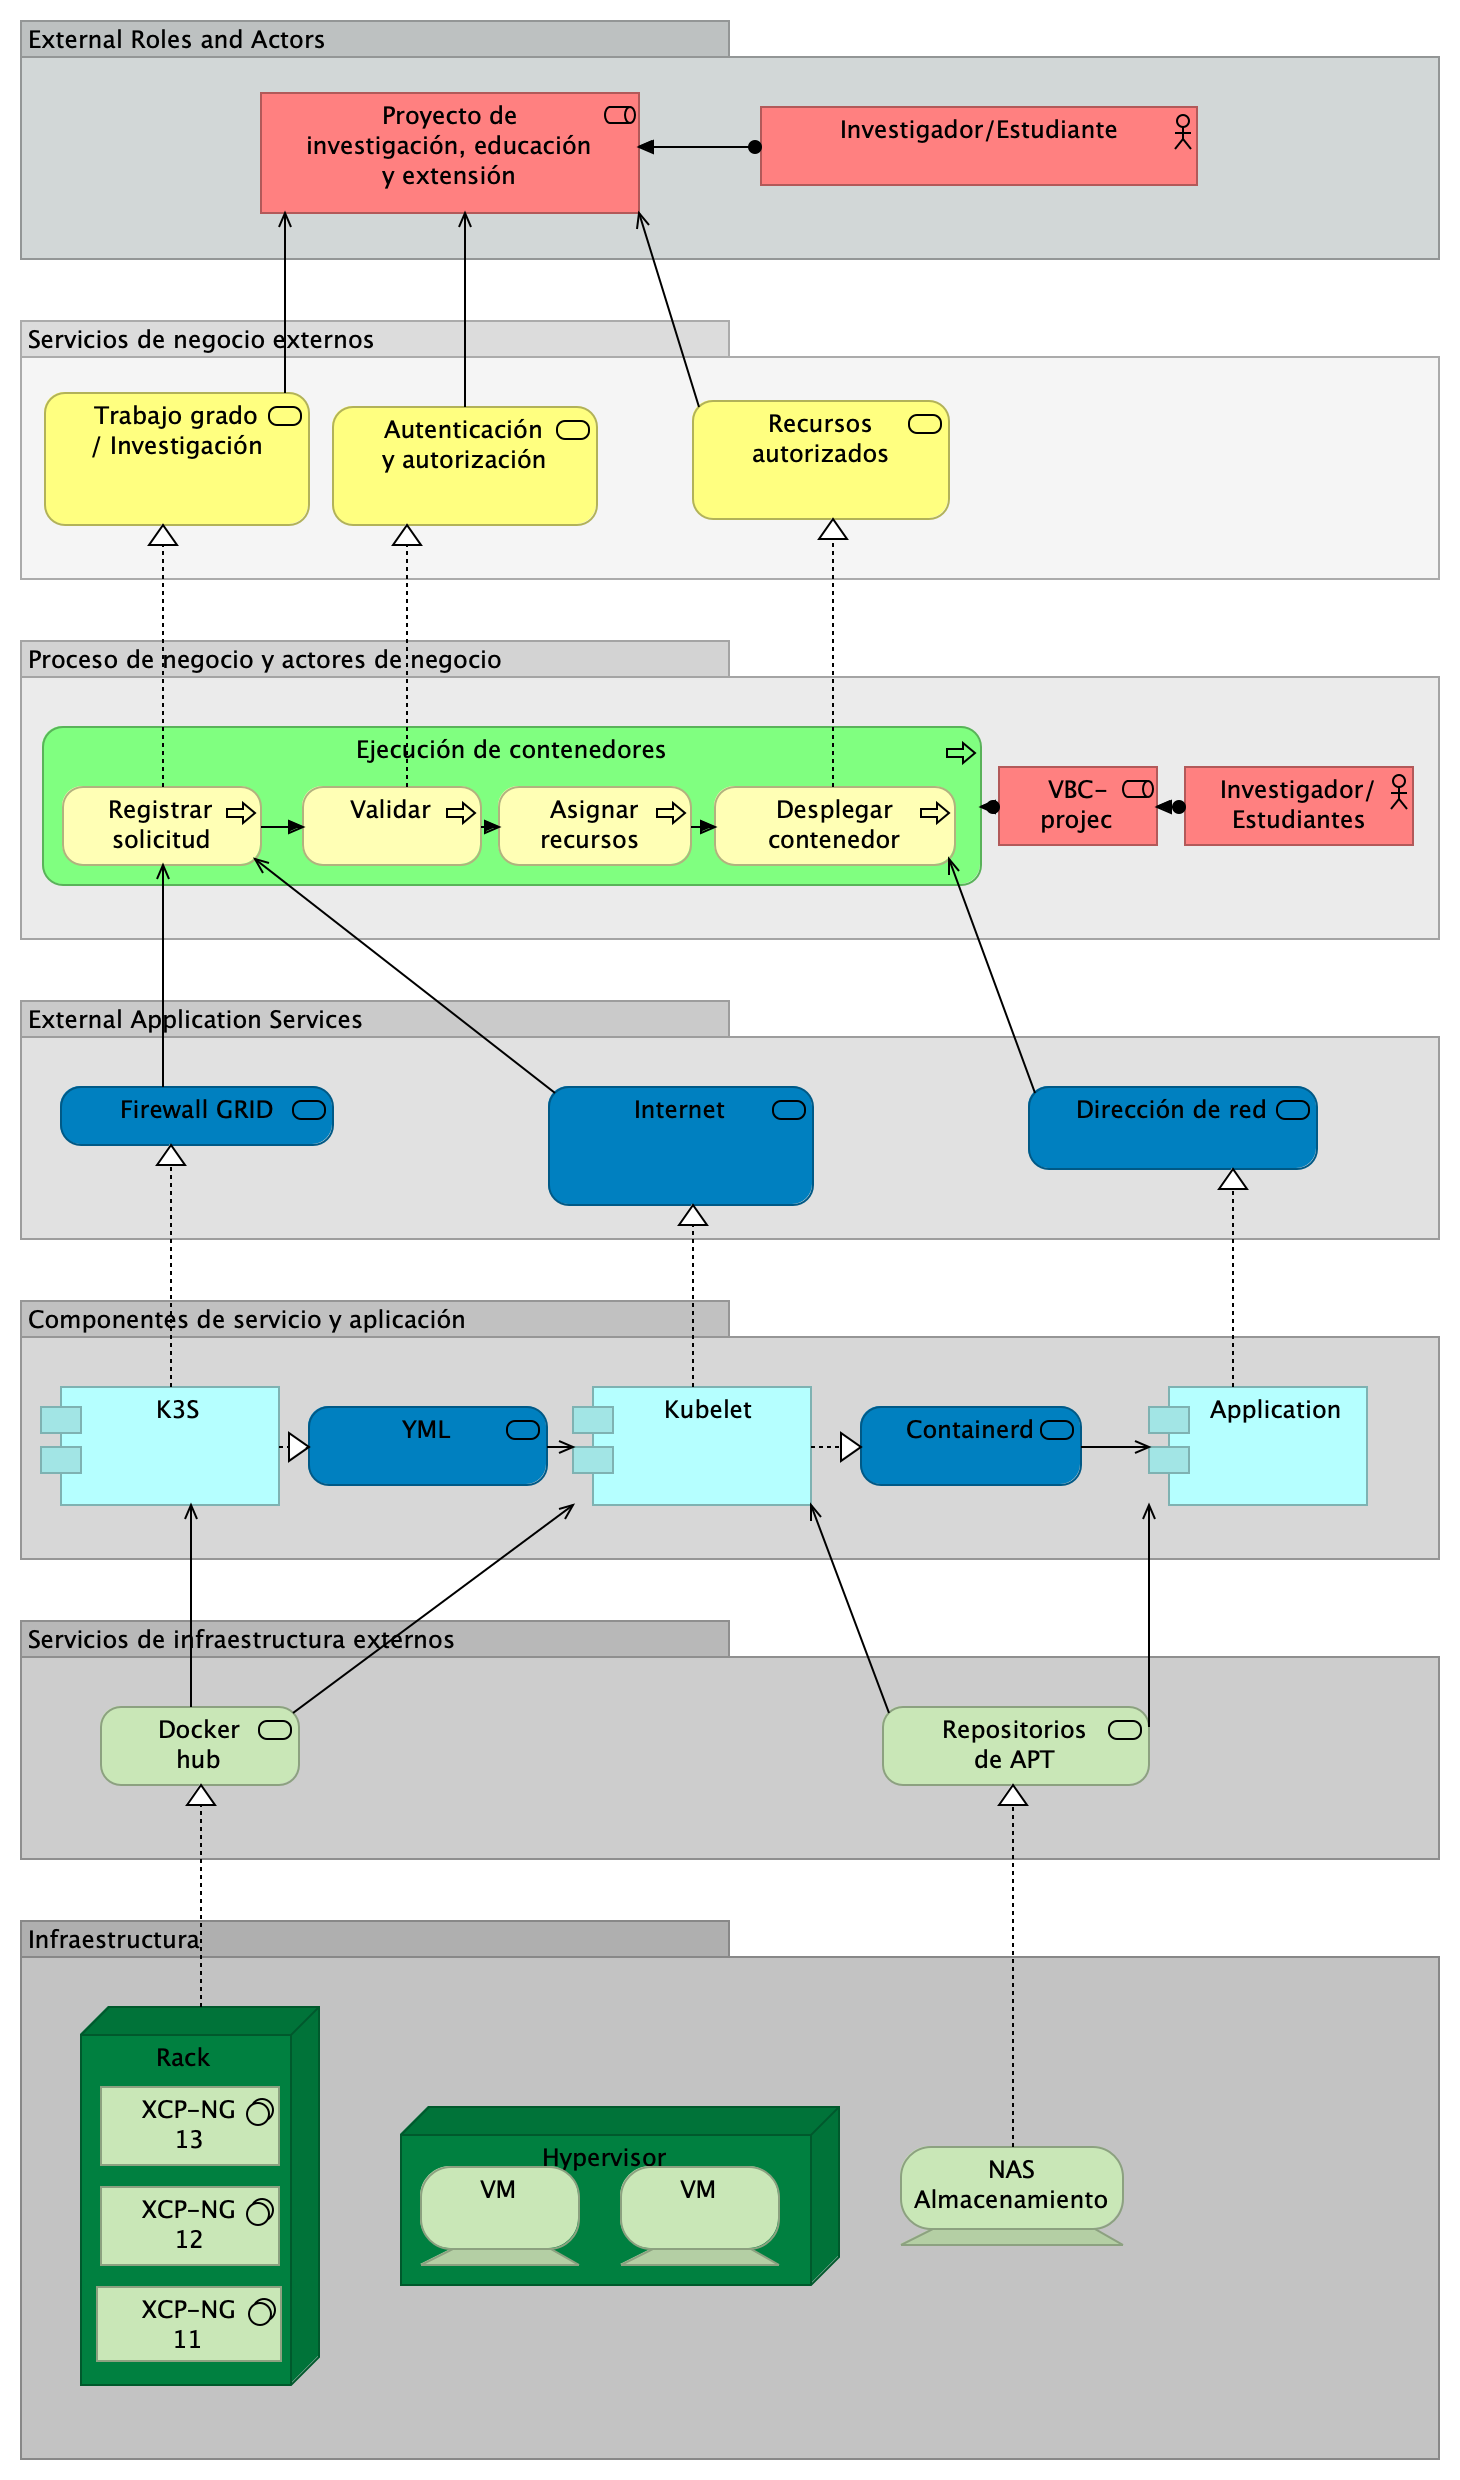
\includegraphics[scale=0.18]{tablas-images/cp6/Layered-View.png}
    \caption{Vista General en Capas}\label{fig:vista-general}
\end{figure}